\documentclass[a4paper,12pt]{article}

%%% Работа с русским языком
\usepackage{cmap}					% поиск в PDF
\usepackage{mathtext} 				% русские буквы в формулах
\usepackage[T2A]{fontenc}			% кодировка
\usepackage[utf8]{inputenc}			% кодировка исходного текста
\usepackage[english,russian]{babel}	% локализация и переносы
\usepackage{xcolor}
\usepackage{hyperref}
 % Цвета для гиперссылок
\definecolor{linkcolor}{HTML}{799B03} % цвет ссылок
\definecolor{urlcolor}{HTML}{799B03} % цвет гиперссылок

\hypersetup{pdfstartview=FitH,  linkcolor=linkcolor,urlcolor=urlcolor, colorlinks=true}

%%% Дополнительная работа с математикой
\usepackage{amsfonts,amssymb,amsthm,mathtools} % AMS
\usepackage{amsmath}
\usepackage{icomma} % "Умная" запятая: $0,2$ --- число, $0, 2$ --- перечисление

%% Номера формул
%\mathtoolsset{showonlyrefs=true} % Показывать номера только у тех формул, на которые есть \eqref{} в тексте.

%% Шрифты
\usepackage{euscript}	 % Шрифт Евклид
\usepackage{mathrsfs} % Красивый матшрифт

%% Свои команды
\DeclareMathOperator{\sgn}{\mathop{sgn}}

%% Перенос знаков в формулах (по Львовскому)
\newcommand*{\hm}[1]{#1\nobreak\discretionary{}
{\hbox{$\mathsurround=0pt #1$}}{}}
% графика
\usepackage{graphicx}
\graphicspath{{pictures/}}
\DeclareGraphicsExtensions{.pdf,.png,.jpg}
\author{Бурмашев Григорий, БПМИ-208}
\title{}
\date{\today}
\begin{document}
\maketitle
\clearpage
\section*{Номер 1}
\[
\int_0^1 dx \int_x^1 dy \int_y^1 e^{z^3} dz 
\]
Делаем подобно 9й таске с семинара (меняем порядок интегрирования):
\begin{center}
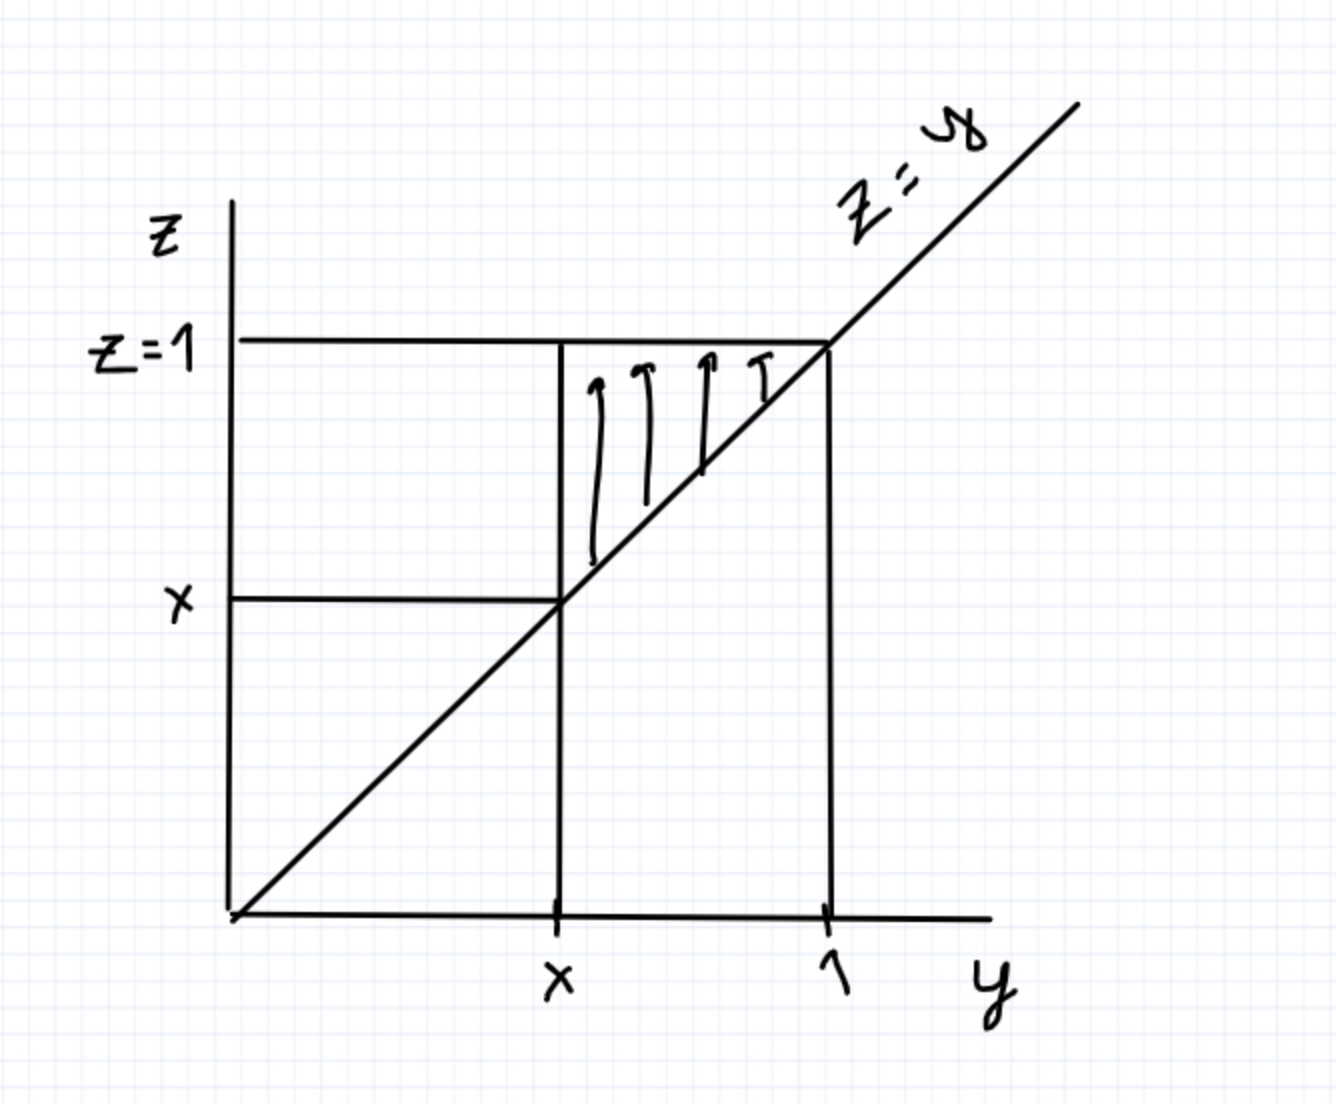
\includegraphics[scale=0.2]{1.png}
\end{center}
\[
\int_0^1 dx \int_x^1 dy \int_y^1 e^{z^3} dz  = \int_0^1 dx \int_x^1 dz \int_x^z e^{z^3} dy =  \int_0^1 dx \int_x^1 e^{z^3} (z - x) dz =
\]
Теперь снова меняем порядок:
\begin{center}

\includegraphics[scale=0.2]{2.png}
\end{center}
\[
=  \int_0^1 dz \int_0^z e^{z^3} (z - x) dx =  \int_0^1  e^{z^3}  dz \int_0^z (z - x) dx = \int_0^1  e^{z^3}  dz \frac{z^2}{2} = \frac{1}{2} \int_0^1  e^{z^3} z^2  dz = 
\]
Пусть $t = z^3,$ отсюда $ dt = 3z^2 dz$, тогда:
\[
 = \frac{1}{2} \cdot \frac{1}{3} \int_0^1 e^t dt =\frac{1}{6} \cdot \left(e^{1^3} - e^{0^3}\right) = \frac{1}{6} \cdot (e - 1) 
\]
\begin{center}
\textbf{Ответ: } 
\[
 \frac{(e-1)}{6} 
\]
\end{center}
\clearpage
\section*{Номер 2}
\[
\iiint\limits_{[0;1]^3} f(x, y, z) dxdydz = 1
\]
Для начала заметим, что функция является симметричной по своим аргументам, т.е $f(x, y, z) = f(x, z, y)$ и т.д
\\\\
Ищем:
\[
\int_0^1 dx \int_0^x dy \int_0^y f(x, y, z) dz 
\]
Для начала заметим, что (пробегаем все значения от 0 до 1):
\[
\iiint\limits_{[0;1]^3} f(x, y, z) dxdydz = 1 = \int_0^1 dx \int_0^1 dy \int_0^1 f(x, y, z) dz 
\]
Так что нам нужно выразить то, что мы ищем через этот интеграл. Пусть то, что мы ищем будет называться $I$
\\
Теперь аналогично предыдущей задаче начнем менять интегралы местами, поменяем $z$ и $y$:
\begin{center}
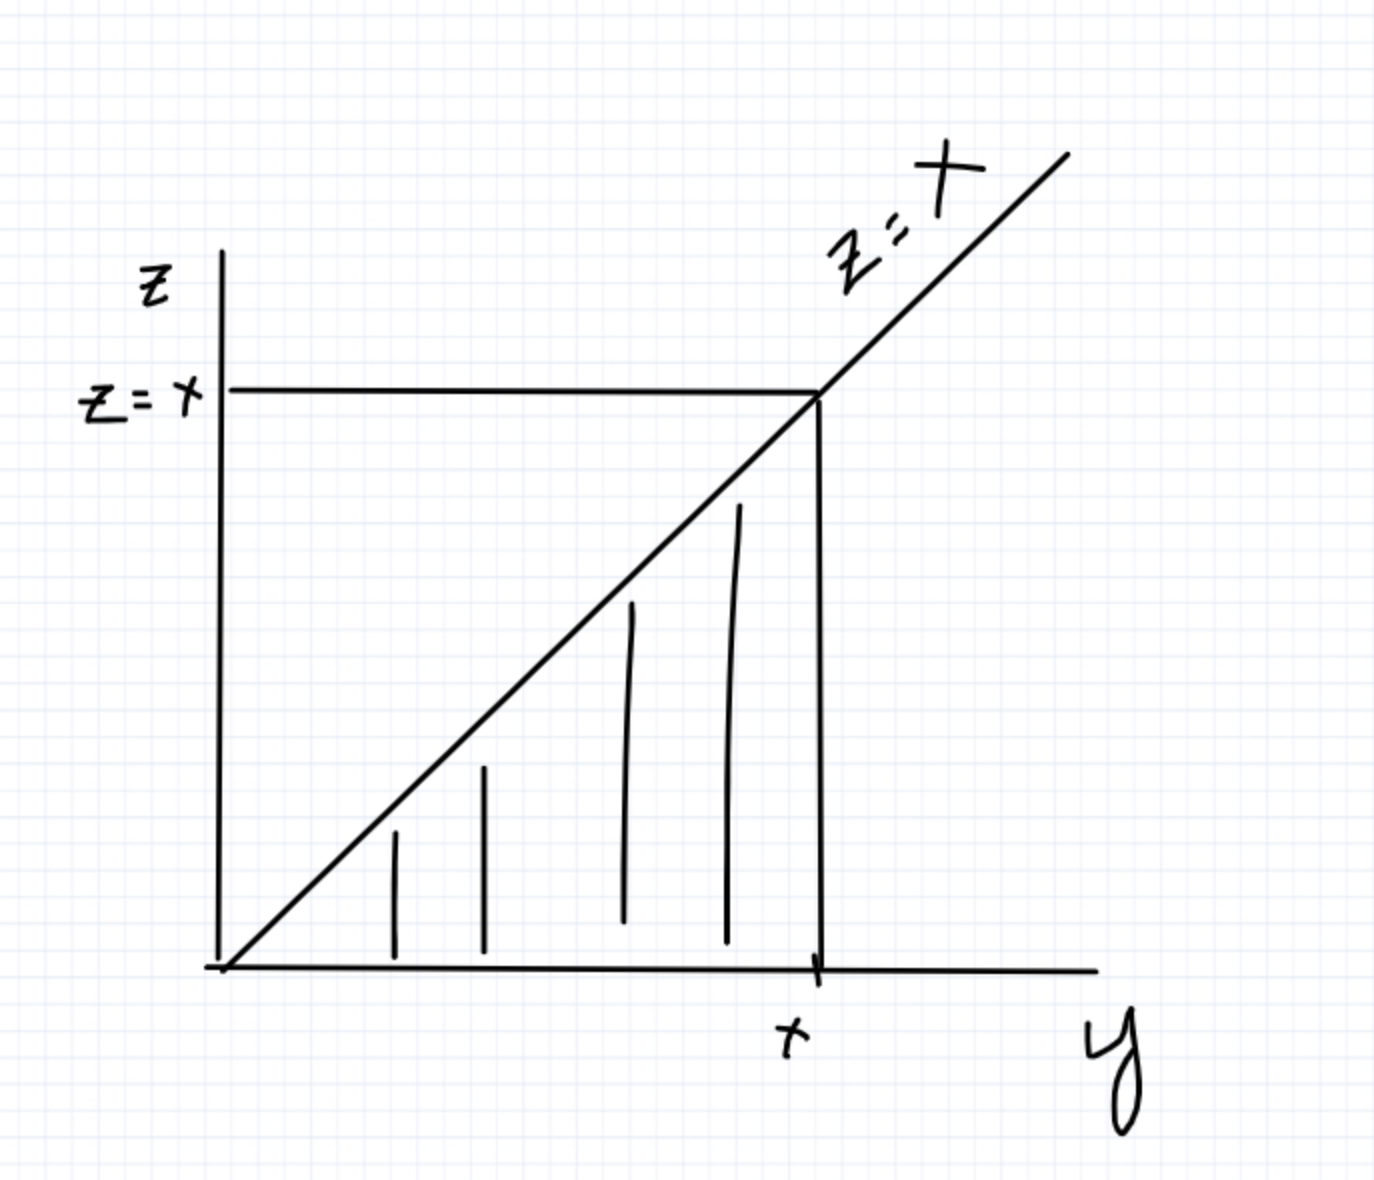
\includegraphics[scale=0.2]{3.png}
\end{center}
\[
I = 
\int_0^1 dx \int_0^x dy \int_0^y f(x, y, z) dz  = \int_0^1 dx \int_0^x dz \int_z^x f(x, z, y) dy  =
\begin{bmatrix}  y = z \\ z = y \end{bmatrix}
=
\]
\[
=
 \int_0^1 dx \int_0^x dy \int_y^x f(x, y, z) dz
\]
Теперь заметим, что полученное похоже на наш исходный интеграл, только внутренний интеграл был $\int\limits_0^y$, а стал $\int\limits_y^x$, тогда если их сложить, то получим сумму от 0 до $y$ и от $y$ до $x$, т.е просто от $0$ до $x$:
\[
2I = \int_0^1 dx \int_0^x dy \int_0^x f(x, y, z) dz  \]
Теперь проделаем ту же операцию, только поменяем $x$ и $y$:
\begin{center}
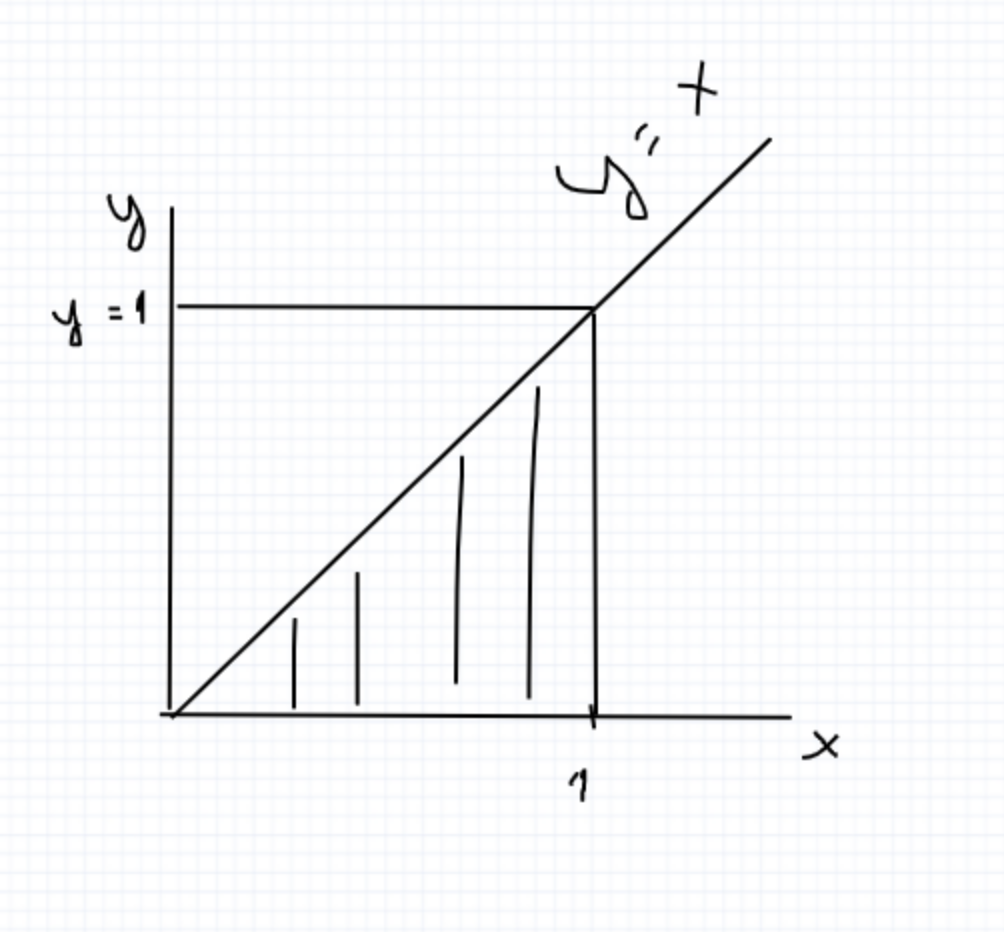
\includegraphics[scale=0.2]{4.png}
\end{center}
\[
I = \int_0^1 dy \int_y^1 dx \int_0^y f(x, y, z) dz = \begin{bmatrix}
x = y \\y = x
\end{bmatrix} = \int_0^1 dx \int_x^1 dy \int_0^x f(x, y, z) dz
\]
Ну и собствено снова складываем, в этот раз полученный выше $2I$ и новый $I$, на этот раз объединятся от $0$ до $x$ и от $x$ до $1$:
\[
3I = \int_0^1 dx \int_0^1 dy \int_0^x f(x, y, z) dz 
\]
Осталось проделать тоже самое с внутренним интегралом, мы еще не меняли местами $x$ и $z$, для этого возьмем $3I$ из того что мы получили выше:
\begin{center}
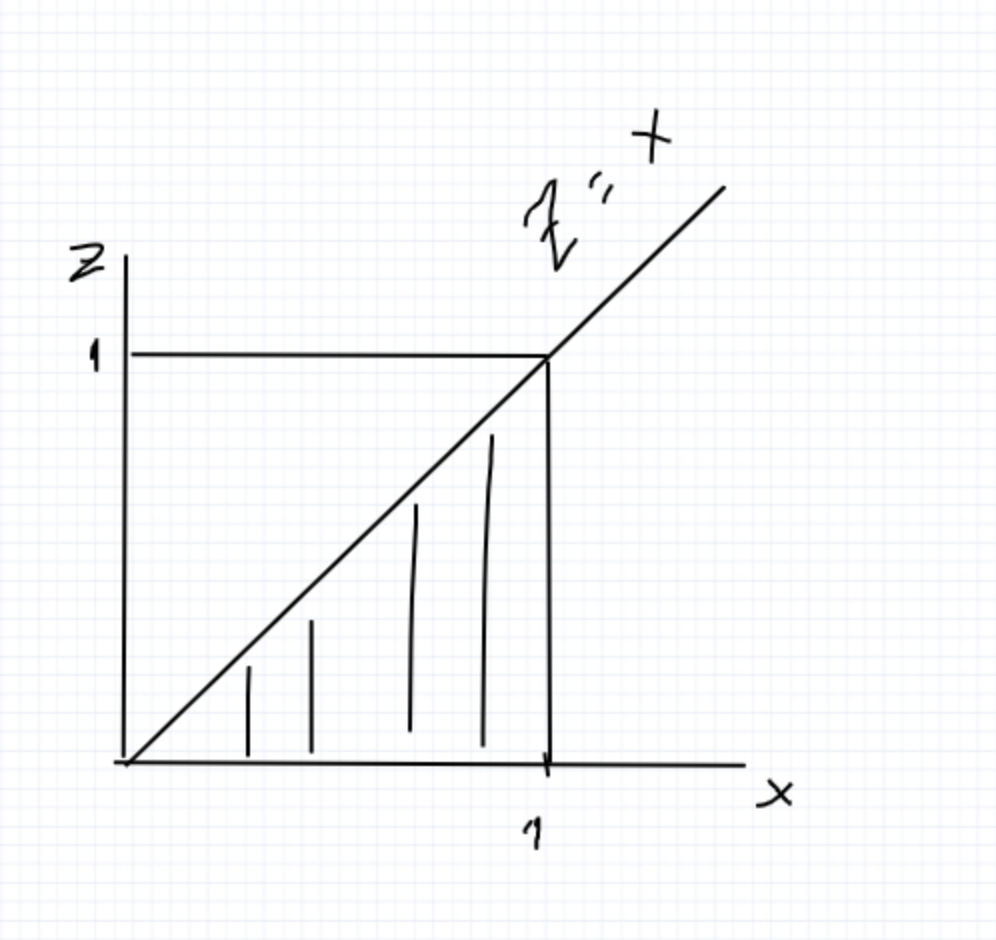
\includegraphics[scale=0.2]{5.png}
\end{center}
\[
3I = \int_0^1 dx \int_0^1 dy \int_0^x f(x, y, z) dz  = \int_0^1 dz \int_0^1 y \int_x^1 f(x, y, z) dx = \begin{bmatrix}
x = z \\
z = x
\end{bmatrix} = 
\]
\[
=
\int_0^1 dx \int_0^1 dy \int_x^1 f(x, y, z) dz
\]
Теперь складываем с формулой $3I$ из второй по счету замены, $0, x$ и $x, 1$ переходят в $0, 1$
\[
6I = \int_0^1dx \int_0^1 dy \int_0^1 f(x, y, z) dz
\]
Ну а по условию задачи и определению это равно единице, т.е:
\[
6I = 1
\]
\[
I =\int_0^1 dx \int_0^x dy \int_0^y f(x, y, z) dz  = \frac{1}{6}
\]
\begin{center}
\textbf{Ответ: } \[
\int_0^1 dx \int_0^x dy \int_0^y f(x, y, z) dz  = \frac{1}{6}
\]
\end{center}
\end{document}
